\section{Stars}

FYI- I looked through the old qual questions we got, and it seems like almost everyone is asked 
something about the HR Diagram, so we should know that inside and out.  Also, questions about 
spectral lines are more popular than I thought they would be.  Globular clusters were also popular.

\subsection{Questions}
\begin{enumerate}
\item \textbf{Explain what is the Hayashi track, and describe what types of objects live on it.
      Qualitatively explain how it arises and what assumptions are required for its derivation.}

\item \textbf{Estimate the temperature as a function of depth in the Sun's convection zone. What is the temperature at the base of the convection zone?}

	%Imagine a blob of gas inside a gaseous medium whose density deviates from the density of its environment. If the blob's density is smaller than the surrounding density, the system is unstable to convection (we should also know how to express this in terms of entropy).
	%Imagine that the blob has $\rho_{b1},~P_{b1},~T_{b1}$, and the surrounding medium has $\rho_1,~P_1,~T_1$. The blob moves up a distance $\delta r$, where the environment has $\rho_2,~P_2,~T_2$, and now the blob has $\rho_{b2},~P_{b2},~T_{b2}$. 
	Assume the process is adiabatic, so the blob obeys $P = K \rho ^\gamma$, and assume we have an ideal gas, so $P = \frac{\rho k_{\rm B} T}{\mu m_p}$. First differentiate the ideal gas law to obtain
	
	\begin{equation}
	\frac{dP}{dr} = \frac{P}{\rho} \frac{d \rho}{dr} + \frac{P}{T} \frac{d T}{dr} \,\, ,
	\end{equation}
	assuming that the pressure does not vary much with the mean molecular weight $\mu$. We can also differentiate the adiabatic pressure equation
	\begin{equation}
	\frac{dP}{dr} = \gamma \frac{P}{\rho}\frac{d\rho}{dr}\,\, .
	\end{equation}
	Setting these two equal, we get
	\begin{equation}
	\biggl(\frac{dT}{dr}\biggr)_{\rm ad} = \biggl(1 - \frac{1}{\gamma}\biggr)\frac{T}{P} \frac{dP}{dr}\,\, ,
	\end{equation}
	which is the adiabatic temperature gradient. In a star, we can also use the ideal gas law to replace $P$ and hydrostatic equilibrium to replace $dP/dr$:
	\begin{equation}\label{conv}
	\biggl(\frac{dT}{dr}\biggr)_{\rm ad} = -\biggl(1 - \frac{1}{\gamma}\biggr)\frac{\mu m_p}{k_{\rm B}} \frac{G M_r}{r^2}\,\, .
	\end{equation}
	This describes how the temperature in the bubble changes as it rises and expands adiabatically. If $dT/dr$ is steeper than the adiabatic temperature gradient, the fluid is superadiabatic and there will be convection.
	
	The convection zone of the Sun extends about $R_\astrosun/3$ down from the surface. Assume $M_r$ is constant and is the mass of the Sun, i.e. relatively little mass is contained in the convection zone. For an ideal monatomic gas, $\gamma = 5/3$, and let's assume $\mu \approx 1/2$, since in the outer layers of the Sun it should be mostly hydrogen. We can integrate our equation to get $T(R)$:
	
	\begin{equation}
	\int^{T(R)}_{T_{\rm eff}} dT = -\frac{m_p}{5 k_{\rm B}} G {\rm M}_\odot \int^R_{\rm R_\odot} r^{-2}dr \,\, .
	\end{equation}
	Alternatively, you could integrate from the base of the convection zone if you know what the temperature is there ($1.8 \times 10^6~K$) and can remember that it's about a third of the way in. The final formula is:
	\begin{equation}
	T(R) = \frac{m_p}{5 k_{\rm B}} G {\rm M}_\odot \biggl( \frac{1}{R} - \frac{1}{{\rm R}_\odot}\biggr) + 5800~{\rm K}\,\, .
	\end{equation}
	And you can plug numbers in yourself (someone check the form of this equation and make sure io got it right).
	
\item \textbf{Describe the major sources of opacity in stars, and how each depends on density,
      temperature, and metallicity.}
      
      \newthought{There roughly four} regimes that are important for determining the
      continuum opacity of the star.  In order of increasing temperature: blending of
      spectral lines, H$^-$ absorption, neutral H absorption, and electron scattering.
      Let's discuss each of these in turn.

      \newthought{At very low temperatures,} (ie. in the atmospheres of M dwarfs and brown dwarfs),
      where $T<3000$ K (I'm guessing at this temperature -- Michael), the number of molecular
      and atomic lines can become overwhelming.  At a certain point, the lines begin to fall
      on top of each other and act as a source of continuum opacity.  At a certain point, the
      opacity becomes so great that it influences the structure of star\sidenote{
        For instance in brown
        dwarfs, the blended line opacity is so great that light escapes the surface of the star
        only in regions where there aren't very many molecular lines.  In the infrared,
        color filters are designed on the same criteria (we don't want atmospheric lines
        contaminating our images).  Therefore, brown dwarfs have almost all of their light
        coming out in bands centered on the color filters Y, J, H, and K.  As a side-effect,
        this also makes brown dwarfs look very blue.
      }.

      Electron scattering (Thomson): This opacity is due to photons scattering off free electrons. This opacity is generally close to constant, since the Thomson cross-section is a constant given by
      \begin{equation}
      \sigma_{\rm T} = \frac{8 \pi e^4}{3 c^4 m_e^2} = 6.6524\times 10^{-25}~{\rm cm}^2\,\, .
      \end{equation}
      The opacity $\kappa = \sigma / m$, so the opacity will depend on the total mass per scattering electron; that is, it will depend on the composition of the material and also how much it is ionized. Because of the ionization state, it will also depend on the temperature, i.e. whether the material is fully ionized. For a fully ionized medium, however, the opacity should be roughly constant, since there will typically be 1 or 2 baryons per electron, so $m \sim 1-2~m_p$. Therefore $\kappa$ is usually of the order 0.1-0.4 cm$^2$ g$^{-1}$.

      The exact opacity (assuming a fully ionized gas) from Thomson scattering can be calculated 
      as a function of H mass fraction.  In a similar calculation to the mean molecular weight 
      derivation, 
      \begin{equation}
      n_e=n_H+2n_{He}+\Sigma{A}{2}n_A=\frac{\rho}{m_H}\left(X+\frac{2}{4}Y+\frac{1}{2}Z\right)=\frac{\rho}{2m_H}\left(1+X\right)
      \end{equation}
      So,
      \begin{equation}
      \kappa_T=\frac{n_e\sigma_T}{\rho}=\frac{sigma_T}{2m_H}\left(1+X\right)=\left(1+X\right)0.2~{\rm cm^2 g^-1}
      \end{equation}
       
      H$^-$ ion: Occasionally, if there are enough free electrons present (easier with increased partial ionization of heavy elements), some will become weakly bound to hydrogen atoms, so that the proton is surrounded by two electrons. Opacity is caused by photoionization of this extra electron with binding energy of 0.75 eV. 
      
      \begin{equation}
      \kappa_{H^{-}} \propto Z \rho^{1/2} T^{9}
      \end{equation}
      
      The opacity is very sensitive to temperature, because a fragile balancing act is required. The temperature must be less than 10,000K (when Hydrogen ionizes) so that neutral Hydrogen is around to get another electron. But, the temperature must also be high enough so that an abundance of free electrons are around which were liberated from ionized heavy elements. This opacity is also sensitive to metallicity, for the same reason. 
      Despite $H^{-}$ being a fragile and rare ion, this type of opacity is the most important source in our Sun's atmosphere, and is dominant in FGK stars.

      Neutral H Transitions:
      These include bound-bound transitions and bound-free transitions.  In bound-bound 
      transitions, a photon is absorbed by an atom, moving an electron to a higher energy level.  
      These transitions have corresponding wavelengths asscociated with them, giving rise 
      to spectral lines.  Higher density leads to higher opacity, but the temperature 
      dependence of this opacity is complicated.  The temperature and composition determine 
      how many atoms of a certain type there are, and what state these atoms are in.  This 
      determines the strengths of spectral lines.  Of course, if the star is hot enough to 
      ionize everything, neutral transitions will not take place.
      
      Bound-free opactiy is the ionization of an atom (H is most important, since it's most 
      abundant).  For photons with enough energy to ionize H, the cross section depends varies 
      as $\lambda^3$.  On our stars midterm, we had to plot bound-free opacity as a function of 
      wavelength.  I can't draw it here, but it's good to know what the plot looks like.  
      Bound-free opacity is responsible for the Balmer jump is stellar spectra at 365 nm, where 
      H in the $n=2$ level can be ionized.  This produces a drop in flux from the star at shorter 
      wavelengths.

      Averaging bound-free and free-free absorption over all wavelenthts gives Kramer's opacity:
      \begin{equation}
      \bar{\kappa}\propto \frac{\rho}{T^{3.5}}
      \end{equation}
       
\end{enumerate}

\subsection{Stellar Properties}
Let's start by listing the properties of the Sun, which are just good to know.
\begin{dgroup}
\begin{dmath}
L_\astrosun = 3.8 \times 10^{33}~{\rm erg}~{\rm s}^-1
\end{dmath}
\begin{dmath}
R_\astrosun = 6.9 \times 10^{10}~{\rm cm}
\end{dmath}
\begin{dmath}
M_\astrosun = 2 \times 10^{33}~{\rm g}
\end{dmath}
\begin{dmath}
t_\astrosun = 4.5 \times 10^9~{\rm yrs}
\end{dmath}
\begin{dmath}
T_{\rm eff} = 5800~{\rm K}
\end{dmath}
\begin{dmath}
T_{\rm c} = 15 \times 10^6~{\rm K}
\end{dmath}
\begin{dmath}
\rho_{\rm c} = 150~{\rm g}~{\rm cm}^{-3}
\end{dmath}
\begin{dmath}
\langle \rho \rangle_\astrosun = 1~{\rm g}~{\rm cm}^{-3}
\end{dmath}
\end{dgroup}
Ranges for other stars:
\begin{dgroup}
\begin{dmath}
M \sim 0.1 - 100~{\rm M}_\astrosun
\end{dmath}
\begin{dmath}
R \sim 0.1 - 1000~{\rm R}_\astrosun
\end{dmath}
\begin{dmath}
L \sim 10^{-4} - 10^6~{\rm L}_\astrosun
\end{dmath}
\begin{dmath}
T_{\rm eff} \sim 1000 - 5 \times 10^4~{\rm K}
\end{dmath}
\end{dgroup}

\subsection{Spectral Types}
O, B, A, F, G, K, M\newline
Within these types, stars are numbered 0 through 9 (hottest to coolest).  Luminosity classes 
are also used.  I-IV are giant stars, while V are main sequence stars.  D is for white dwarfs.  
So, for example, the Sun is a G2V star.\newline
O stars:\newline
>16 $M_{\odot}$, $M_V=-5$ or brighter\newline
Very weak spectral lines (just about everything is ionized, so there's nothing 
to produce transitions).  Very weak Balmer lines and some weak lines to due 
ionization of He.  No Balmer break visible.\newline
B stars:\newline
2-16 $M_{\odot}$\newline
Stronger Balmer lines, also He absorption lines.  Still a relatively clean 
spectrum though.  Balmer break visible (and visible in all later spectral 
types.\newline
A stars:\newline
1.5-2 $M_{\odot}$, $M_V\sim 0$\newline
Strongest Balmer lines because these are the hottest stars (hot enough to have 
lots of H in the n=2 state) without being too hot and ionizing all the H.  
Effective temperature of $\sim$10,000 K is perfect for Balmer lines.\newline
F stars:\newline
1-1.5 $M_{\odot}$\newline
Balmer lines start to weaken again.  Star seeing metal lines (mainly neutral 
or singly ionized Ca, Mg, and Na).\newline
G stars:\newline
0.8-1 $M_{\odot}$, $M_V\sim4$\newline
This includes the Sun.  Weaker Balmer lines, stronger metal lines.\newline
K stars:\newline
0.5-0.8 $M_{\odot}$\newline
Weaker Balmer, stronger metal.  Also start seeing absorption bands from 
molecules (smearing of lots of absorption lines due to rotational, vibrational, 
and electronic transitions).
M stars:\newline
<0.5 $M_{\odot}$, $M_V\sim 8-12$\newline
Dominated by molecular bands, in particular TiO between 6600\AA\ and 8600\AA.

\subsection{HR Diagram}
Be able to draw and explain one.  Some useful approximate relations for the main sequence:
\begin{equation}L\propto T_{eff}^8\end{equation}
\begin{equation}R\propto T_{eff}^2\end{equation}
\begin{equation}L\propto M^3\ for\ stars\ more\ massive\ than\ the\ Sun\end{equation}
\begin{equation}L\propto M^5\ for\ stars\ less\ massive\ than\ the\ Sun\end{equation}
Main sequence masses range from $\sim 0.1\ M_{\odot}$ to $\sim 100\ M_{\odot}$.  Main sequence 
radii range from $\sim 0.25\ R_{\odot}$ to $\sim 25\ R_{\odot}$.  Temperatures range from 
around $2000-3000\ K$ to $\sim 50,000\ K$.  Luminosities range from $\sim10^{-3}L_{\odot}$ to 
$\sim500,000-1,000,000L_{\odot}$ (somebody should check these ranges, they're estimates/pulled 
from Wikipedia).  

Since the energy of a star comes from its mass, main sequence lifetimes can be estimated as
\begin{displaymath}
\tau_{ms}\sim\frac{E}{L}\sim\frac{M}{L}\sim M^{1-\alpha}
\end{displaymath}
where $\alpha$ is given by the mass-luminosity relation.  So, for stars more massive than the 
Sun,
\begin{equation}
\tau_{ms}\sim M^{-2}
\end{equation}
and for stars less massive than the Sun,
\begin{equation}
\tau_{ms}\sim M^{-4}
\end{equation}
Anything less massive than the Sun basically lives forever.

\subsection{Equations of Stellar Structure}
\newthought{There are three} key pieces of physics that are necessary for understanding stars:
\begin{enumerate}
    \item Force balance: pressure vs. gravity (and sometimes rotation)
    \item Energy transport: conduction, radiation, convection
    \item Energy generation: fusion, gravitational contraction
\end{enumerate}
These form the essence of the equations of stellar structure.
\begin{dgroup*}
\begin{dmath}
    \frac{\d M_r}{\d r} = 4\pi r^2\rho \quad \text{(mass continuity)}
\end{dmath}
\begin{dmath}
    \frac{\d P}{\d r} = -\frac{GM_r\rho}{r^2} \quad \text{(hydrostatic equilibrium)}
\end{dmath}
\end{dgroup*}

Let's talk first about force balance. Assuming no radiation, this is just a competition between pressure and gravity. We can look at a layer in the star with pressure $P$ at its base and $P+dP$ above, and we know the force on the layer due to gravity. The total force will be the pressure difference times the area of the shell $A$ (which will eventually drop out) plus the gravitational force $-\frac{G M_r M_{\rm shell}}{r^2}$. If we assume hydrostatic equilibrium, the total force is zero. We then can switch to differentials to get the hydrostatic equilibrium equation:

\begin{equation}
\frac{dP}{dr} = -\frac{\rho G M_r}{r^2}\,\,.
\end{equation}

The mass continuity equatin just comes from the amount of mass in a spherical shell at radius r 
and of thickness dr.

The radiative temperature gradient can be derived by considering the energy in shells at different 
radii.  Since energy flows out of the star, the energy density must decrease outwards.  Consider 
a shell with energy denstity $u+du$ (shell 1), with another shell $dr$ above it of energy 
density $u$ (shell 2).  The energy flow from shell 1 to shell 2 per unit time ($L(r)$) is 
the excess energy in shell 1 divided by the time it takes for this energy to flow from shell 1 to 
shell 2.  So
\begin{equation}\label{eq:L}
L(r)=-\frac{4\pi r^2\,dr\,du}{(dr)^2/lc}
\end{equation}
where the denominator is the time it takes a the photon to cross from shell 1 to shell 2 by random 
walk.  Taking the angle of the radiation into account introduces a factor of 1/3 on the right hand 
side.  Equation \ref{eq:L} can be rewritten as 
\begin{equation}
\frac{L(r)}{4\pi r^2}=-\frac{cl}{3}\frac{du}{dr}
\end{equation}
This can also be thought of as a diffusoin equation, where the left hand side is energy flux, 
$\frac{cl}{3}$ is the diffusion coefficient, and $\frac{du}{dr}$ is the energy density gradient.  
Plugging in $u=aT^4$ and $l=\frac{1}{\kappa\rho}$, and solving for $\frac{dT}{dr}$ gives
\begin{equation}\label{eq:rad}
\boxed{\frac{dT(r)}{dr}=-\frac{3L(r)\kappa(r)\rho(r)}{4\pi r^2 4acT^3(r)}}
\end{equation}

The energy conservation equation just comes from defining $\epsilon(r)$ as the power generated 
per unit mass.  With this definition,
\begin{equation}
\boxed{\frac{dL(r)}{dr}=4\pi r^2\rho (r)\epsilon (r)}
\end{equation}

In addition to the four main equations of stellar structure, three more equations must be 
specified for the pressure, opacity, and energy generation.  
\begin{equation}
P=P(\rho,T,composition)
\end{equation}
\begin{equation}
\kappa=\kappa(\rho,T,composition)
\end{equation}
\begin{equation}
\epsilon=\epsilon(\rho,T,composition)
\end{equation}
Also, the four differential equations require four boundary conditions:
\begin{equation}
M(r=0)=0
\end{equation}
\begin{equation}
L(r=0)=0
\end{equation}
\begin{equation}
P(r=R)=0
\end{equation}
\begin{equation}
M(r=R)=M_*
\end{equation}

So, there are 7 equations for 7 unknowns, and 4 boundary conditions for 4 differential equations.  
This means that there is a unique solution given the composition and total mass of the star, the 
only two free parameters in the equations.  This is the \emph{Vogt-Russell conjecture}, that the 
properties and evolution of a star depend only on its mass and initial composition.

The equation of state is almost always ideal gas, but here's a good derivation of mean molecular 
weight, which I personally can never remember.

For a fully ionized gas, H contributes 2 particles, He contributes 3, and metals contribue 
$\sim\frac{A}{2}$.  So the total number density of particles is
\begin{equation}
n=2n_H+3n_{He}+\Sigma \frac{A}{2}n_A=\frac{rho}{m_H}\left(2X+\frac{3}{4}Y+\frac{1}{2}Z\right)=\frac{\rho}{2m_H}\left(3X+\frac{1}{2}Y+1\right)
\end{equation}
using the fact that $X+Y+Z=1$.  Then
\begin{equation}
\mu=\frac{\rho}{nm_H}=\frac{2}{1+3X+0.5Y}
\end{equation}

io likes the following definition of mean molecular weight:
\begin{equation}
\frac{1}{\mu_I} = \sum \frac{X_i}{A_i}\,\, ,
\end{equation}
\begin{equation}
\frac{1}{\mu_e} = \sum \frac{Z_iX_i}{A_i} \,\, ,
\end{equation}
\begin{equation}
\frac{1}{\mu} = \biggl(\frac{1}{\mu_I} + \frac{1}{\mu_e} \biggr)^{-1}\,\,.
\end{equation}

See the will ask question for a discussion of opacity.

Also, radiation pressure can contribute to the overall pressure (and sometimes dominate).  
For a photon gas,
\begin{equation}
P_{rad}=\frac{1}{3}u=\frac{1}{3}aT^4
\end{equation}

\subsection{The Hayashi Track}
\newthought{The Hayashi track}
describes the evolution of star that is entirely convective
(with a narrow radiative envelope for the photosphere).
Hayashi derived these tracks by showing that for
a given mass, there is an effective temperature below which no stable solutions exist.
That is, any star with an effective temperature below the limit will collapse until its
effective temperature is above the limit.  In this way, stars essentially slide along
the boundary of stability, maintaining a constant effective temperature
(even as their central temperature increases).

Let's see a brief derivation of this.  To begin with we assume that the interior is entirely
convective so that the pressure is given by the adiabatic relationship
\begin{dmath}
    P\propto\rho^\gamma
\end{dmath},
By combining this with the ideal gas law, we find that
\begin{dmath}\label{eq:pt_adiabatic}
    P\propto T^{\frac{\gamma}{\gamma-1}}
\end{dmath}.
For a monatomic gas, $\gamma=5/3$, so that $P\sim T^{5/2}$.

Next we can use the equation of hydrostatic equilibrium to estimate the central pressure $P_c$ and
temperature $T_c$ as\sidenote{
    To see this, approximate $\d P/\d r$ as $P_c/R$ and approximate $\rho$ as $M/R^3$.
    Forget about numerical constants because we're just looking for a scaling relationship
    here.  The temperature comes from the ideal gas law.
}:
\begin{dgroup*}
\begin{dmath*}
    P_c \sim \frac{M^2}{R^4}
\end{dmath*}
\begin{dmath*}
    T_c \sim \frac{M}{R}
\end{dmath*}
\end{dgroup*}
With these expressions for the central pressure and temperature, we can use
Equation~\ref{eq:pt_adiabatic} to find the pressure and temperature anywhere in the
star -- notably at the surface of the photosphere.

However, before we can do that, we need to locate the photosphere.  To do this, we
assume an opacity law of the form $\kappa \sim \rho T^a$, and that the photosphere
can be treated in the plane-parallel approximation\sidenote{
    This assumes that the photosphere is narrow and contains a negligible amount of mass.
}.
In this case the equation of hydrostatic equilibrium becomes
\begin{dmath*}
\frac{\d P}{\d z} = -\rho g
\end{dmath*},
where $g = GM/R^2$.  The photosphere is located where $\tau\sim 1$ (or $\tau\sim 2/3$ if
you're being picky), so let's replace $\d z$ with the optical depth $\d\tau = -\kappa\rho\d z$
such that
\begin{dmath*}
\frac{\d P}{\d\tau} = \frac{g}{\kappa}
\end{dmath*}.
Integrating to the surface of the photosphere therefore gives us
\begin{dmath}
    P_{\rm eff} \sim \frac{g}{\kappa} \nolinebreak
                \sim \frac{R}{T_{\rm eff}^a}
\end{dmath}.
Using Equation~\ref{eq:pt_adiabatic} and our expressions for $P_c$, $T_c$, and $P_{\rm eff}$
we can solve for $T_{\rm eff}$ to find (taking $\gamma=5/3$)
\begin{dmath}\boxed{
    T_{\rm eff} \sim R^{2.5/(2.5+a)}M^{0.5/(2.5+a)}
}\end{dmath}.
Therefore when the opacity is very temperature sensitive\sidenote{
    For H$^-$ opacity, $a\sim10$.
}, the effective temperature is almost independent of radius.  Therefore the Hayashi
track is a vertical line on the HR diagram.

It is worth noting here that it is critical for the opacity to increase rapidly with temperature.
As the star contracts, the central temperature of the star increases.  In fact, at any fixed
position within the star, the temperature increases.  However, if the opacity is very temperature
sensitive, the photosphere will stay at a location where the temperature remains roughly
constant.  This means that the effective temperature stays constant.

\subsection{The Henyey Track}

\newthought{In the core}
of a protostar, Kramer's opacity law is a good description of the mean opacity.
As the protostar contracts along the Hayashi track, the temperature of the core increases
even as the effective temperature remains constant.  The opacity in the core therefore decreases
as the star contracts and eventually the core becomes radiative.  As the star continues to
contract, the opacity in the core further decreases and the radiative region grows in size.
Therefore the structure of the star responds to further contraction by lowering the opacity
in its core and moving more energy through radiation.  This allows the star to push more energy
out (it's more transparent to radiation!), and hence the luminosity increases.  Because the
luminosity is increasing while the radius is shrinking, the effective temperature must also
increase (it can no longer remain constant as on the Hayashi track)\sidenote{
    Recall that $L=4\pi R^2\sigma T_{\rm eff}^4$ to good approximation.
}.  Therefore, when the core becomes radiative, the protostar moves to higher luminosities and
higher effective temperatures (after moving to lower luminosities with a constant effective
temperature on the Hayashi track).  This track is occasionally called the Henyey track.

\indent The relation between luminosity, mass, and T$_{eff}$ for objects on the Henyey track can be derived with homology, using the following scaling relations which apply to the core of the protostar:

\begin{enumerate}
	\item Kramer's opacity: $\kappa \propto \rho T_{c}^{-3.5}$
	\item Ideal gas: $P \propto \rho T_{c}$, where $\rho \propto M R^{-3}$
	\item Radiative energy transport\sidenote{This scaling relation comes from solving for $\kappa$ in Equation \ref{eq:rad}, and approximating $dT(r)/dr$ as $T/R$}: $\kappa \propto T_{c}^{4} L^{-1} M^{-1} R^{4}$
\end{enumerate}

\noindent Finally, by using everyone's favorite $L \propto R^{2} T_{eff}^{4}$, you find that

\begin{equation}
L \propto M^{22/5} T_{eff}^{4/5}
\end{equation}

This equation illustrates what was described above -- as the core becomes radiative, an increase in $L$ corresponds to an increase in $T_{eff}$.

\newthought{Cool note} on the Henyey Track -- if the mass of the protostar is too low, then hydrogen burning ignites before the events which cause the protostar to travel along the Henyey track can begin.  Thus, the resulting main sequence star will remain completely convective -- this is why main sequence stars with mass $< .8 M_{\odot}$ are fully convective (and why their Hayashi tracks directly intersect the main sequence, without the upward trend of the Henyey track; see Figure 2.2 in HKT for a good plot illustrating this).  

\subsection{Scaling Relations on the Main Sequence}
Assume that P(r), M(r), $\rho (r)$, and T(r) are roughly power laws.  Then from the equations of stellar structure we have:

\begin{equation}
P \thicksim \frac{\rho M}{r}
\end{equation}
\begin{equation}
M \thicksim r^3\rho
\end{equation}
\begin{equation}
L \thicksim \frac{T^4r}{\kappa \rho}
\end{equation}

For moderately massive stars greater than $1 M_\odot$, the pressure is dominated by kinetic gas pressure and the opacity is dominated by electron scattering.

\begin{equation}
P \thicksim \rho T
\end{equation}
\begin{equation}
\kappa = constant
\end{equation}

Equating hydrostatic equilibrium with the equation of state:

\begin{equation}
P \thicksim \frac{M\rho}{r} \thicksim \rho T
\end{equation}
\begin{equation}
T \thicksim \frac{M}{r}
\end{equation}

Replacing T in the luminosity equation yeidls:
\begin{equation}
L \thicksim M^3
\end{equation}

Furthermore, $M \thicksim R$ on the main sequence, which implies a constant core temperature.  To see this, consider a star that is contracting and heating up.  An equilibrium will be established when the density and the temperature in the core are high enough for the onset of nuclear reactions.  Since the nuclear power density $\epsilon$ depends mainly on temperature, for any initial mass, the radius of the star will stop shrinking when a particular core temperature is reached.  Therefore the internal temperature is comparable in all main sequence stars.  From stellar models, over a range of around 100 in mass, the core temperature varies only by a factor of 4.  

For stars less massive than the sun, the opacity is dominated by bound-bound and bound-free opacities, which follow kramer's opacity $\kappa \thicksim \rho T^{-3.5}$.  Since the temperature is approximately constant:

\begin{equation}
 M \thicksim R
\end{equation}
\begin{equation}
\kappa \thicksim \rho \thicksim \frac{M}{r^3} \thicksim M^{-2}
\end{equation}

The luminosity equation becomes:

\begin{equation}
L \thicksim \frac{M}{M^{-2}M^{-2}} \thicksim M^{5}
\end{equation}

For the most massive stars, radiation pressure dominates.  The equation of state then goes as $P \thicksim T^4$, and electron scattering opacity dominates.  The mass-luminosity relationship then goes as:

\begin{equation}
L \thicksim M
\end{equation}





\subsection{Stellar Evolution}

Collapse from a gas cloud:

The first important thing to know is the Jeans criterion. You can get here by considering a deviation from a system in hydrostatic equilibrium, which is described by the Virial Theorem:

\begin{equation}
2K + U = 0\,\, ,
\end{equation}
where we can approximate the kinetic and gravitational potential energies as

\begin{equation}
U \sim \frac{3 G M_{\rm c}^2}{5 R_{\rm c}}
\end{equation}
\begin{equation}
K = \frac{3}{2} N k_{\rm B} T = \frac{3 M_{\rm c} k_\rm B T}{\mu m_{\rm H}}
\end{equation}

You can assume a constant density for the cloud and find the minimum mass necessary to start collapse, $M_{\rm c} > M_{\rm J}$:

\begin{equation}
M_{\rm J} \approx \biggl( \frac{5 k_{\rm B}T}{G \mu m_{\rm H}}\biggr)^{3/2}\biggl( \frac{3}{4\pi\rho_0}\biggr)^{1/2}
\end{equation}

We can also express this criterion as $R_{\rm c} > R_{\rm J}$, where

\begin{equation}
R_{\rm J} \approx \biggl( \frac{15 k_{\rm B} T}{4 pi G \mu m_{\rm H} \rho_0} \biggr)^{1/2}
\end{equation}

Once the Jeans criterion is satisfied, the cloud basically collapses in freefall at the beginning. It is isothermal, optically thin, and radiates energy efficiently. The freefall time is

\begin{equation}
t_{\rm ff} = \biggl( \frac{3 \pi}{32 G \rho_0}\biggr)^{1/2} \sim \biggl( \frac{1}{G \rho_0}\biggr)^{1/2}
\end{equation}
The numerical factor is from the derivation in Carrol \& Ostlie; you can derive this by considering a particle on the outer edge of and object falling inward due to the gravitational force of all the interior mass.

Also note that fragmentation is an issue: that is, the Jeans mass changes as the density of the cloud goes up, and a natural consequence of this is that a smaller mass is required to collapse. Therefore, one large cloud (of, say, 50 solar masses) might collapse into $\sim 50$ solar-mass clouds.

What eventually stops fragmentation is that the cloud stops being isothermal. The cloud starts transporting more energy adiabatically rather than radiatively because it starts to become optically thick, and radiation does not transport energy out efficiently enough.

(There is some stuff about shocks produced by the outer layers of the cloud free-falling onto the nearly hydrostatic star, which powers it for a while. Not sure how much we need to know about this.)

To see that fragmentation must stop, use the fact that the collapse becomes 
adiabatic.  So
\begin{equation}
T\propto\rho^{\gamma-1}
\end{equation}
Plugging this into the Jeans mass expression gives
\begin{equation}
M_J\propto\rho^{(3\gamma-4)/2}
\end{equation}
For $\gamma=5/3$, this gives $M_J\propto\rho^{1/2}$, so the Jeans mass 
increases with increasing density, which stops fragmentation.

As a fragmented clump collapses, it must have a way of releasing the energy from the collapse, or 
the temperature and pressure will rise and stop the collapse.  At this stage, the excess energy 
goes into first dissociating H$_2$, then ionizing atomic H.  Once (almost) all the H has been 
ionized, the star must release its gravitational energy by radiating.  This slows the collapse, 
and a slowly contracting proto-star forms, with contraction governed by the Kelvin-Helmholtz 
timescale.  

Pre-Main-Sequence Evolution:

First, the \textbf{pre-MS protostar} collapses on the Kelvin-Helmholtz timescale $t_{\rm KH}$, which for $1~{\rm M}_\astrosun$ is about $10^7$ years. The Kelvin-Helmoholtz timescale is given by
\begin{equation}
t_{\rm KH} \approx \frac{GM^2}{RL}\,\, .
\end{equation}
This just comes from approximating the energy available for the luminosity is the gravitational potential energy, so the timescale for radiating this energy is just the total gravitational potential energy divided by the luminosity.

The effective temperature increases, so the opacity of the outer layers becomes dominated by the H$^-$ ion, which gets its extra electrons from increased partial ionization of heavy elements. This increased opacity causes the envelope of the protostar to become convective and sometimes this envelope can become very large, reaching even to the center of the star. This object evolves along the Hayashi track, its luminosity decreasing while the effective temperature increases only slightly (it is almost constant, $\sim 3800$ K).

A \textbf{solar mass star on the Hayashi track} is completely convective and starts burning deuterium in the first million years, which slows the collapse slightly and for a short time, since deuterium is not very abundant. The central temperature rises, and opacity in the center decreases, so the core becomes radiative. This causes the luminosity to start increasing. At the same time, the core becomes hot enough to start more nuclear reactions (dominated by the first two steps of the PP chain and the CNO cycle. Nuclear energy generation starts dominating over luminosity from gravitational collapse. A large temperature gradient develops in the core, which starts to become partly convective again, and then the core expands a bit, which decreases the luminosity because $\epsilon_{\rm grav}$ becomes negative, and $\epsilon = \epsilon_{\rm nuc} + \epsilon_{\rm grav}$. When C-12 is exhausted, the core adjusts and PP-I chain dominates, and the star settles onto the main sequence.

For \textbf{lower-mass stars}, the temperature might never get hot enough to burn C-12, so they don't turn up as much in luminosity, but rather fall closer to the Hayashi track down onto the Main Sequence. Below about 0.08 M$_\odot$, no nuclear reactions can be sustained, and these stars never reach the Main Sequence. Lower mass starts also never develop radiative cores, so they are always fully convective.

\textbf{Massive stars} start burning carbon and hydrogen much more quickly because the central temperature rises faster. These break away from the Hayashi track earlier and at higher luminosities, since nuclear reactions contribute more to the luminosity earlier on. The CNO cycle becomes the dominant energy generation process because of the high temperatures. As the star travels horizontally on the HR diagram, the core remains convective because the energy generation is so temperature-dependent, while the envelope is radiative.

Main Sequence Evolution:

Low mass stars (the mass of the Sun or smaller) increase slightly in luminosity and temperature 
during their main sequence lifetimes.  This is due to the conversion of H to He in the core, 
increasing the mean molecular weight.  This reduces the pressure in the core (ideal gas law), 
causing the core to contract.  The gravitational energy released heats the surrounding material, 
allowing the H burning region to include more material.  Also, the increased temperature and 
density increases the rate of the pp chain.  As a result, the energy output of the core increases, 
increasing the overall luminosity of the star.  The energy released in contraction also goes 
into increasing the effective temperature.  This process causes the star to move up and to the 
left in the HR diagram.  As the H in the core of the star is depleted, an 
inert He core forms, with H shell burning around it.  This shell burning increases the luminosity 
of the star further, and also expands the outer layers, cooling the star.  The star now moves 
up and to the right in the HR diagram.  In stars more massive than the Sun, a convective 
core prevents this process from happening, as new material is brought into the burning region and 
He is removed.  As the star evolves, the convection in the core decreases and there is some 
buildup of He, although not as much as in lower mass stars.  

In high and low mass stars, main sequence evolution ends when too much He builds up in the core.  
The He core is isothermal and does not generate energy, so it must support itself with a density 
gradient.  Once the core reaches around 10\% the mass of the entire star, it will no longer 
be able to support itself or the material above it (note- in very low mass stars, electron 
degeneracy may set in before this happens.  I'm guessing this is how a He white dwarf would form). 
In higher mass stars, when star runs out of H, the entire star contracts, releasing graviational 
energy.  This increases luminosity, while the decrease in radius increases effective temperature.  

Post-Main Sequence Evolution:

This section makes a lot more sense with an HR diagram to refer too, so I'll be referring to the 
figures on page 458 and 459 of Carroll and Ostlie.  Solar mass and intermediate mass stars 
evolve similarly after the main sequence, although the shapes of their tracks are slightly 
different.  At this point, the star has an isothermal He core with H shell burning around it.  
The first stage in post-MS evolution is the \emph{subgiant branch}.  When the He core 
can no longer support itself, it contracts on a Kelvin-Helmholtz timescale, releasing energy and 
increasing luminosity.  The envelope of the star expands, lowering the effective temperature, and 
the star moves up and to the right on the HR diagram (labeled SGB).  As the star's envelope 
expands and cools, the opacity increases due to H$^-$.  This causes a convection zone to form, 
extended from surface of the star to most of the interior.  This convection transport energy from 
the interior to the surface more efficienty, causing a rapid increase in luminosity as the moves 
up the \emph{red giant branch} (RGB).  The path of the RGB is essentially the Hayashi track in 
reverse, which makes sense because both tracks deal with fully convective objects.  During this 
phase, convection brings products of nuclear burning such as C and N from the interior to the 
surface, where they can be seen spectroscopically (dredge-up).  This provides a test for stellar 
evolution models.  When a star reaches the tip of the RGB, the center becomes hot enough to begin 
fusing He through triple-$\alpha$.  The ignition of He expands the core and pushes the H burning 
shell outwards, cooling it and decreasing the rate of energy production.  Shell burning still 
supplies most of the star's luminosity, so the luminosity decreases rapidly (the dotted line on 
page 458).  The envelope of the star contracts during this process, causing the effective 
temperature to rise.   

In stars below $1.8\ M_{\odot}$, the ingition of He creates a \emph{He core flash}.  Before 
ignition starts, the He core is already degenerate.  Once He ignition happens, the energy released 
goes into lifting the degeneracy pressure, instead of expanding and cooling the core.  This leads 
to explosive He burning in the core, producing $10^{11}$ L$_{\odot}$ for a few seconds.  Most of 
this energy is absorbed by the outer layers of the star, so the luminosity on the HR diagram is 
not affected.  

The next step in post-main sequence evolution is the \emph{horizontal branch}.  The H burning 
shell continues to contract, with the increase in density causing an increase in energy output.  
This increases the effective temperature of the star, and the stars moves horizontally to the left 
on basically a He burning main sequence.  What follows is analogous to the subgiant and red giant 
branches.  The mean molecular weight in the He burning core increases, causing it to contract.  
The evelope expands and cools, moving the star to the right on the HR diagram.  As the 
H burning shell expands and cools, it turns off, leaving He burning to power the star.  
When the He in the core runs out, a He burning shell forms and the star moves up the 
\emph{asymptotic giant branch} (AGB).  It becomes convective and there is a second dredge-up 
phase.  Near the top of the AGB, the H burning shell re-ignites and dominates the stars 
luminosity.  The H burning shell begins dumping He onto the He burning layer, increasing its mass 
and making it degenerate.  This leads to periodic He flashes in the shell, which push out the 
H burning layer, cooling it and turning it off.  The luminosity of the star drops until the H 
shell re-ignites, and the process repeats.  Mass loss from the star during this phase can 
reach $10^{-4} M_{\odot}$ per year, due to the pulsations and the formation of high opacity dust 
grains in the cool, loosely bound outer layers of the star.  This forms an optically thick cloud 
of material around the star.  As this cloud continues to expand, it eventually becomes optically 
thin, and the hot core of the star is exposed.  This causes the observed effective temperature 
to increase, moving the star into the \emph{post-AGB} phase.  The expelled envelope becomes a 
planetary nebula and the core becomes a white dwarf, moving down the HR diagram onto the white 
dwarf sequence.  

So, as a quick summary of all this, the basic picture is a star's H runs out, the core 
contracts and the envelope expands as a H burning shell forms.  The star gets brighter and cooler, 
moving to the right and up.  The star becomes convective and moves up a vertical, Hayashi-like 
track.  Then the star starts burning He and settles onto a He main sequence until the He runs out 
and a He burning shell forms.  The core contracts, the envelope expands, and the star gets brighter 
and cooler, moving to the right and up.  The star becomes convective again and Hayashis (that 
should totally be a verb) vertically.  Finally, it blows off it's outer layers and the core 
becomes a C+O white dwarf.

I couldn't find a detailed section on post-MS evolution for massive stars, but I assume it's 
basically the same, just with additional burning stages all the way up to burning Si into Fe, 
which each stage happening faster.


\subsection{Radial Velocities}

Derivation of radial velocity amplitude from a star and a low mass companion (say a planet).

Let $r_p$ be the distance between the planet and the center of mass of the system, and $r_s$ be the distance between the star and the center of mass.

\begin{equation}
a = r_p + r_s
\end{equation}

\begin{equation}
v_p = \frac{2\pi r_p}{P}
\end{equation}
\begin{equation}
v_s = \frac{2\pi r_s}{P}
\end{equation}

\begin{equation}
M_pr_p = M_sr_s
\end{equation}

Combining above equations yields the following relation:
\begin{equation}
\frac{v_p}{v_s} = \frac{r_p}{r_s} = \frac{M_s}{M_p}
\end{equation} 

\begin{equation}
a = r_p + r_s = (\frac{M_s}{M_p} + 1)r_s = r_s\big(\frac{M_s + M_p}{M_s}\big)
\end{equation}

Plugging the above expression into Kepler's 3rd law:

\begin{equation}
P^2 = \frac{4\pi^2r_s^3(M_p + M_s)^2}{GM_p^3}
\end{equation}

Plugging in for $r_s$ and rearranging a bit:

\begin{equation}
v_s^3 = \frac{P^{-1}2\pi GM_p^3}{(M_p + M_s)}
\end{equation}

By assuming the companion is significantly less massive than the star, you can simplify the expression for the radial velocity amplitude K.  
\begin{equation}
v_s = K = 2\pi G P^{-\frac{1}{3}}M_pM_s^{-\frac{2}{3}}
\end{equation}

\subsection{Atmospheres}
The Boltzmann and Saha equations are probably more involved than we need to know (especially the 
Saha equation), but here they are anyway.
\begin{equation}
\frac{n_1}{n_2}=\frac{g_1}{g_2}e^{-(E_1-E_2)/kT}
\end{equation}
\begin{equation}
\frac{n_{i+1}}{n_i}=\frac{2Z_{i+1}}{n_eZ_i}\left(\frac{2\pi m_ekT}{h^2}\right)^{3/2}e^{-\chi_i/kT}
\end{equation}
where $n_{i+1}$ and $n_i$ are are the numbers of atoms in the $i$ or $i+1$ ionization state, 
$Z_i$ is the partition function of the $ith$ ionization state, and $\chi_i$ is the ionization 
energy.  All we should probably know for these equations relating to stars is that the describe 
the population of atoms in the star's atmosphere, and thus determine the strengths of spectral 
lines.  For example, the competing temperature dependence of these equations gives that the 
peak fraction of H atoms in the $n=2$ state happens at around 10,000 K.  This is why A stars show 
such strong Balmer lines.

Optical Depth and the atmosphere:
Using the radiative transfer equation with simplifying assumptions (plane-parallel atmosphere, 
wavelength independent opacity (grey), and the Eddinton approximation- the intensity of radiation 
is just an average of outward and inward radiation), can show that (see Carroll and Ostlie pg 
258-263) the temperature in the 
atmosphere varies with optical depth as:
\begin{equation}
T^4=\frac{3}{4}T_{eff}^4\left(\tau_{\nu}+\frac{2}{3}\right)
\end{equation}
This equation implies that the photosphere (where $T=T_{eff}$) is at $\tau=2/3$.  This also 
explains spectral lines and limb darkening.  If a certain wavelength corresponds to an atomic 
transition, that wavelength will have a higher opacity than the continuum.  So the point 
where $\tau=2/3$ will be higher in the star at that wavelength (in other words, you can't 
see as deep into the star at that wavelength).  Because of this, the light we see at that 
wavelength comes from cooler gas than light from the continuum, so there is less flux at that 
wavelength.  Limb darkening is the same idea.  At the edge of the disk of a star, we look into 
the atmosphere at an angle from the verticle direction, so $\tau=2/3$ is higher in the atmosphere, 
and thus cooler, so we see less flux from it.  In both cases, the effective temperature at 
$\tau=2/3$ is cooler.

Spectral Lines:
Spectral lines are broadened by natural broadening, Doppler broadening, and pressure broadening.  
Natural broadening is due to the uncertainty principle.  Since an electron spends a short time 
in an excited state, there is an uncertainty the energy of the state.  This makes the wavelenght 
of light that can be absorbed uncertain.  The typcial full-width-half-max of natural broadening is 
of the order of $10^{-5}nm$.  Doppler broadening is due to random thermal motions of the gas 
described by the Maxwell-Boltzmann distribution.  In the Sun, with $T_{eff}=5777 K$, the 
full-width-half-max of this effect is $\sim 10^{-2}$ nm.  Large-scale motions, such as turbulence, 
rotation, mass loss, and pulsation also contribute to Doppler broadening.  Doppler broadening 
is wider than natural broadening, but falls off exponentially, much faster than natural 
broadening (so the center line shape is due to Doppler broadening, but the wings are shaped by 
natural and pressure broadening.  Pressure broadening is caused when collisions of individual 
particles and electric fields of large numbers of particles perturb the energy levels of atoms.  
Pressure broadening has a similar shape and full-width-half-max to natural broadening.

\subsection{Interiors}
Most of this is covered in the stellar structure equations section.  The only other thing I can
think of is polytropes.  Maybe just some basic knowledge of them would be good (enough to 
answer that question Shri kept asking us in stars about what it means for white dwarfs or 
protostars to have a certain polytropic index).

\subsection{Homology}

Homology is used to find scaling relations between properties of a star, e.g. $R(M), L(M), P_{c}(M), T_{c}(M)$ to name a few.  We must first determine four things about the star we are considering:

\begin{enumerate}
	\item Is pressure given by ideal gas ($P \propto \rho T$) or radiative pressure support ($P \propto T^{4}$).
	\item Is the luminosity carried by radiative diffusion ($\kappa \propto T^{4} L^{-1} M^{-1} R^{4}$)\sidenote{This scaling relation comes from solving for $\kappa$ in Equation \ref{eq:rad}.} or convection ($T \propto M R^{-1}$)\sidenote{From the adiabatic temperature gradient, Equation \ref{conv}}.
	\item Is Thomson ($\kappa \propto \rho^{0} T^{0}$) or Kramer's opacity ($\kappa \propto \rho T^{-3.5}$) dominating.
	\item Through what process is fusion occurring, e.g. p-p chain ($\epsilon \propto \rho T^{4}$) or CNO cycle ($\epsilon \propto \rho T^{15}$).
\end{enumerate}

Then, using the equations of \textbf{mass continuity}

\begin{equation}
\rho \propto \frac{M}{R^{3}}
\end{equation}

\noindent and \textbf{hydrostatic equilibrium}

\begin{equation}
P \propto \frac{M \rho}{R}
\end{equation}

\noindent and the \textbf{energy conservation} equation

\begin{equation}
L \propto R^3 \rho \epsilon
\end{equation}

\noindent we can set up a system of equations to solve for whatever scaling relation we desire for the star.


\subsection{Nuclear Energy Generation}

Nuclear reactions are the primary power source in stars -- for stars on the main sequence, it is the fusion of four hydrogen nuclei into one $^{4}$He.  For fusion to occur, an atomic nucleus must overcome the Coulomb barrier of another nucleus into the potential well created by the strong nuclear force which binds nuclei together.

In the classical picture, the ability of a particle to overcome the Coulomb barrier is determined by whether the thermal energy is greater than the Coulomb potential energy.  The temperature $T_{classical}$ required to overcome the barrier can be estimated using the following equation\sidenote{This doesn't take into account the fact that the Maxwell-Boltzmann distribution of velocities will give some of the particles much higher velocities than $v_{avg}$ and therefore much higher thermal energies.  But this gives a good general picture of why we need quantum mechanics to describe nuclear reactions!}:

\begin{equation}
\frac{3}{2} k T_{classical} = \frac{Z_{1} Z_{2} e^2}{r}
\end{equation}

\begin{equation}
T_{classical} \sim 10^{10} \text{  K}
\end{equation}

\noindent assuming the collision is between two protons and $r$ is the radius of a typical nucleus ($10^{-10}$ cm).  Since the Sun's central temperature is on the order of $10^7$ K, there would not be a sufficient number of particles with high enough thermal energies to overcome the Coulomb barrier and thereby power the Sun.

The answer is (\textit{clearly}) quantum mechanical tunneling, whereby the inherent uncertainty in the position of the particle is large enough that even though there is not enough kinetic energy in the collision of two particles, one can still wind up in the potential well of the other and allow fusion to proceed.

The probability of successful tunneling (and a nuclear reaction occurring) is related to the ratio of the Coulomb barrier height to the initial kinetic energy of the incoming nucleus (this can be visualized by associating a \textit{larger} ratio with a \textit{wider} barrier and therefore a lower probability of tunneling -- see Figure 10.4 in Carroll and Ostlie).  Specifically, the probability for penetrating the Coulomb barrier is 

\begin{equation}
g(E) = e^{-\sqrt{E_{G}/E}}
\end{equation}

\noindent where $E$ is the particle kinetic energy and $E_{G}$ is the Gamow energy\sidenote{$\alpha=\frac{e^2}{\hbar c} = \frac{1}{137}$ is the fine structure constant and $\mu$ is the reduced mass.}:

\begin{equation}
E_{G} = \left(\pi \alpha Z_{1} Z_{2} \right)^2 2 \mu c^2
\end{equation}


The probability for a nuclear reaction, however, will depend not only on the probability of penetrating the Coulomb barrier, but on the nuclear cross section, which should scale as $1/E$.  The cross section is

\begin{equation}
\sigma(E) = \frac{S(E)}{E} g(E) =  \frac{S(E)}{E} e^{-\sqrt{E_{G}/E}}
\end{equation}

\noindent where $S(E)$ is some function which varies very slowly as a function of energy, so we can write it as a constant\sidenote{Sometimes, $S(E)$ does not hold constant, but peaks rapidly at specific energies that correspond to energy levels within the nucleus due to the resonance between the nucleus' energy level differences and the energy of the incoming particle.  This resonance phenomenon is important in the triple-alpha process.}.

The rate of nuclear reactions (number of reactions per time per volume) is given by 

\begin{equation}
R_{AB} = n_{A} n_{B} \sigma_{AB} v_{AB}.
\end{equation}

If the average energy per reaction $\Delta mc^2 = Q_{AB}$, then the energy generation (power per unit mass) is 

\begin{equation}\label{engen}
\epsilon = \frac{Q_{AB} R_{AB}}{\rho} = Q_{AB} \frac{n_{A} n_{B}}{\rho} \left<\sigma_{AB} v_{AB}\right>.
\end{equation}

We want to average $\sigma_{AB} v_{AB}$ over all velocities, where the distribution of velocities is given by the Maxwell-Boltzmann distribution\sidenote{Even though we're in the center of a star and the gas is really hot, the MB distribution still applies because our nuclei still constitute a classical, (nuclei are massive and slow) non-relativistic gas.}.  Therefore, we get that

\begin{equation}
\left< \sigma_{AB} v_{AB} \right> = \int_0^{\infty} \sigma_{AB} v_{AB} P(v_{AB}) dv_{AB}
\end{equation}

where

\begin{equation}
P(v)dv = 4 \pi \left( \frac{\mu}{2 \pi kT} \right)^{3/2} v^2 \exp\left(- \frac{\mu v^2}{2kT}\right) dv
\end{equation}

The point of all this, and probably the only relevant thing we need to know for the qual\sidenote{Being able to draw that plot below is also probably pretty good.}, is that after changing velocity in the above integral to kinetic energy (using $E = \frac{1}{2} \mu v^2$), the integrand becomes

\begin{equation}\label{gamp}
f(E) = e^{-E/kT} e^{-\sqrt{E_{G}/E}}.
\end{equation}

This function is referred to as the Gamow peak and is the product of the Maxwell-Boltzmann high-energy exponential tail (first term) and the Coulomb barrier penetration probability\sidenote{That's what she said.} (second term).

\begin{figure}[h!]
\begin{center}
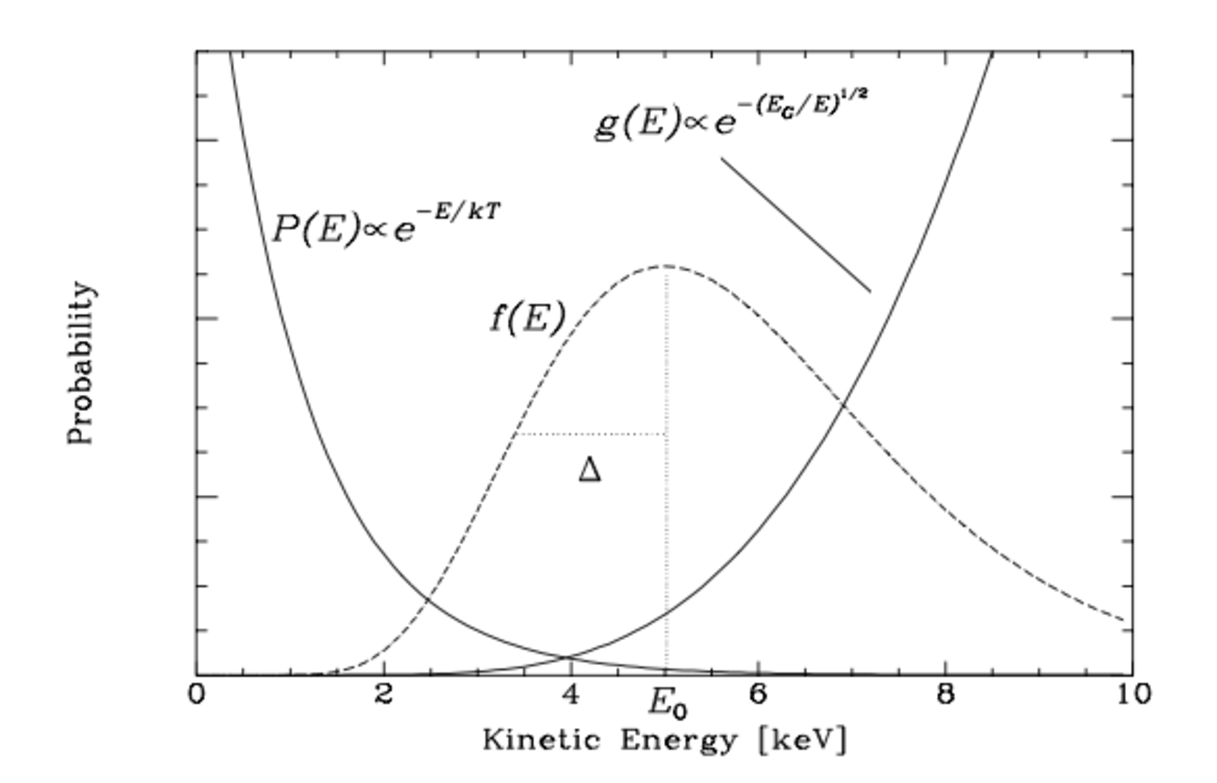
\includegraphics[width=.9\textwidth]{gamow_peak.pdf}
\end{center}
\end{figure}

This curve describes the range of kinetic energies over which nuclear reactions will take place.  The maximum is found by setting the derivative of Equation \ref{gamp} equal to zero, and thus

\begin{equation}
E_{o} = \left( \frac{kT}{2} \right)^{2/3} E_{G}^{1/3}.
\end{equation}

The greatest contribution to the nuclear reaction rate comes from a narrow energy band that depends on the temperature of the gas $T$, and the masses and charges of the reacting nuclei ($\mu$ and $Z_{1},Z_{2}$).

The energy generation rate, $\epsilon$ in Equation \ref{engen}, can then be found by doing some fancy math.  The important part is that it contains an exponential term that goes as 

\begin{equation}
\epsilon \propto \exp \left[ -3 \left( \frac{E_{G}}{4kT}\right)^{1/3} \right]
\end{equation}

Because of the Gamow energy in the exponential, there will be a strong preference for reactions between species with low atomic number, and thus small $E_{G}$; e.g., for similar abundances of deuterium and carbon in the center of star with kinetic energies typical of the Sun (1 keV), the p-p chain reactions would be heavily favored over the CNO cycle (see below for explanations of these reactions).

Also, the steep temperature dependence of nuclear reactions works as a "thermostat" in stars.  If $T$ increases inside a star, the rate of nuclear reactions will increase, $L$ will increase, the star will expand, which will cause $T$ to decrease, and the rate of nuclear reactions will decline accordingly.  Over the lifetime of the star, once the dominant nuclear fuel runs out, the rate of nuclear reactions will go down, the core will contract, and $T$ will rise until a new nuclear reaction involving nuclei of higher atomic number becomes favored\sidenote{This text is from Astrophysics in a Nutshell, pg. 57}.

\newthought{The following} are some relevant nucleosynthesis chains.  In each chain of the reactions, the following conservation laws must hold: conservation of electric charge, number of nucleons, and number of leptons\sidenote{The only way I can remember what constitutes a lepton is remembering that it means "light thing".  It includes electrons, positrons, neutrinos, and antineutrinos.}.

\begin{table}[h!]
\centering
\begin{tabular}{c c c}
\hline\hline
Reaction&$\gamma$&$\nu$\\
\hline
p-p & 1 & 4\\
CNO & 1 & 15\\
triple-$\alpha$ & 2 & 40\\
\hline\hline
\end{tabular}
\caption{Summary table for energy generation for various reactions, where $\epsilon \propto \rho^{\gamma} T^{\nu}$.}
\end{table}
 
 \begin{enumerate}
 \item \textbf{Proton-Proton Chain}: Chain of reactions which convert hydrogen to helium.
 
 \begin{equation}
 ^1_1H + \text{}^1_1H \rightarrow \text{}^2_1H + e^{+} + \nu_{e}
 \end{equation}
 \begin{equation}\label{ppstep2}
 ^2_1H + \text{}^1_1H \rightarrow \text{}^3_2He + \gamma
 \end{equation}
 \begin{equation}
 ^3_2He + \text{}^3_2He \rightarrow \text{}^4_2He + 2\text{}^1_1H
 \end{equation}
 
 The first step is the slowest because it involves the decay of a proton into a neutron (weak force).  There are two other p-p chain branches; the second p-p chain involves the interaction of the helium-3 produced in Equation \ref{ppstep2} with a helium-4 ($^7Be$ and $^7Li$ are intermediate products).  The third p-p chain involves the capture of an electron by the $^7Be$ nucleus created in the second p-p chain.  Most solar neutrinos come from the first p-p chain, but the highest energy ones come from the third p-p chain, despite this having a very low probability of occurrence.
 
 Important note: the total amount of energy released in forming the helium nucleus (binding energy) from four protons is $E_{b} = \Delta mc^2 = 26.731$ MeV.  That is, the combined mass of the four hydrogen atoms is greater than the mass of the resulting helium atom by $\Delta m = 26.731\text{MeV}/c^2$, or $0.7\%$ -- i.e. why hydrogen fusion has an efficiency factor of $.007$.
 
 \item \textbf{CNO Cycle}: This is another cycle for producing helium-4 from hydrogen.  The CNO cycle is more strongly temperature-dependent than the p-p chain, and is the dominant method of generating helium from hydrogen in massive stars ($\geq 1.2 M_{\odot}$) which have higher central temperatures (compared to low-mass stars, which predominantly use the p-p chain).  The CNO cycle uses carbon, nitrogen, and oxygen as catalysts and like the p-p chain has multiple branches\sidenote{I am too lazy to type them all out here, they are on pg. 311 in Carroll and Ostlie}.
 
Note: when hydrogen is converted into helium by either the p-p chain or the CNO cycle, the mean molecular weight $\mu$ of the gas increases, which (from the ideal gas law) means the central pressure will decrease.  That stellar core, no longer being in hydrostatic equilibrium, will begin to collapse.  This has the effect of raising the central temperature and density to compensate for the increase in $\mu$; once the temperature and density are high enough, helium nuclei can overcome their Coulomb repulsion and begin to fuse.\sidenote{This text is from Carroll and Ostlie pg. 312.  This page also has more information on the CNO cycle.}.
 
 \item \textbf{Triple-$\alpha$ Process}: This is the chain of reactions in which helium is converted into carbon-12.
 
 \begin{equation}
 ^4_2He + \text{}^4_2He \rightleftharpoons \text{}^8_4Be
 \end{equation}
 \begin{equation}
 ^8_4Be + \text{}^4_2He \rightarrow \text{}^{12}_6C + \gamma
 \end{equation}
 
 The beryllium nucleus produced by step one is unstable (even-numbered A) and will rapidly decay back into two heliums if it does not immediately interact with another helium nucleus.  The resonance of $^8_4Be + \text{}^4_2He$ with the energy of an excited state of carbon-12 greatly increases the probability of this second step occurring.
 \end{enumerate}